\section{Halbleiter}
\subsection{Grundlagen}
Leitfähigkeit $\kappa$, Elementarladung $q = 1.6\cdot10^{-19}$ As zur Ladungsdichte $n$ und Beweglichkeit der Ladungsträger $\mu$.
\[
\kappa = \frac{1}{\varrho} = nq\mu
\]

Widerstand $R$ eines Materialsstücks mit Länge $l$, Querschnitt $A$ und der Materialkonstante $\varrho$:
\[
R = \rho \cdot \frac{l}{A} = \frac{l}{\kappa \cdot A}
\]

Temperaturabhängigkeit
\[
\varrho(T) = \varrho(T_0) \cdot (1 + \alpha(T - T_0))
\]

\includegraphics[width=\columnwidth]{Images/leitfähigkeit}

\subsection{Diode}
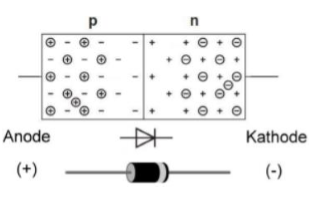
\includegraphics[width=0.4\columnwidth]{Images/diode_grafik}

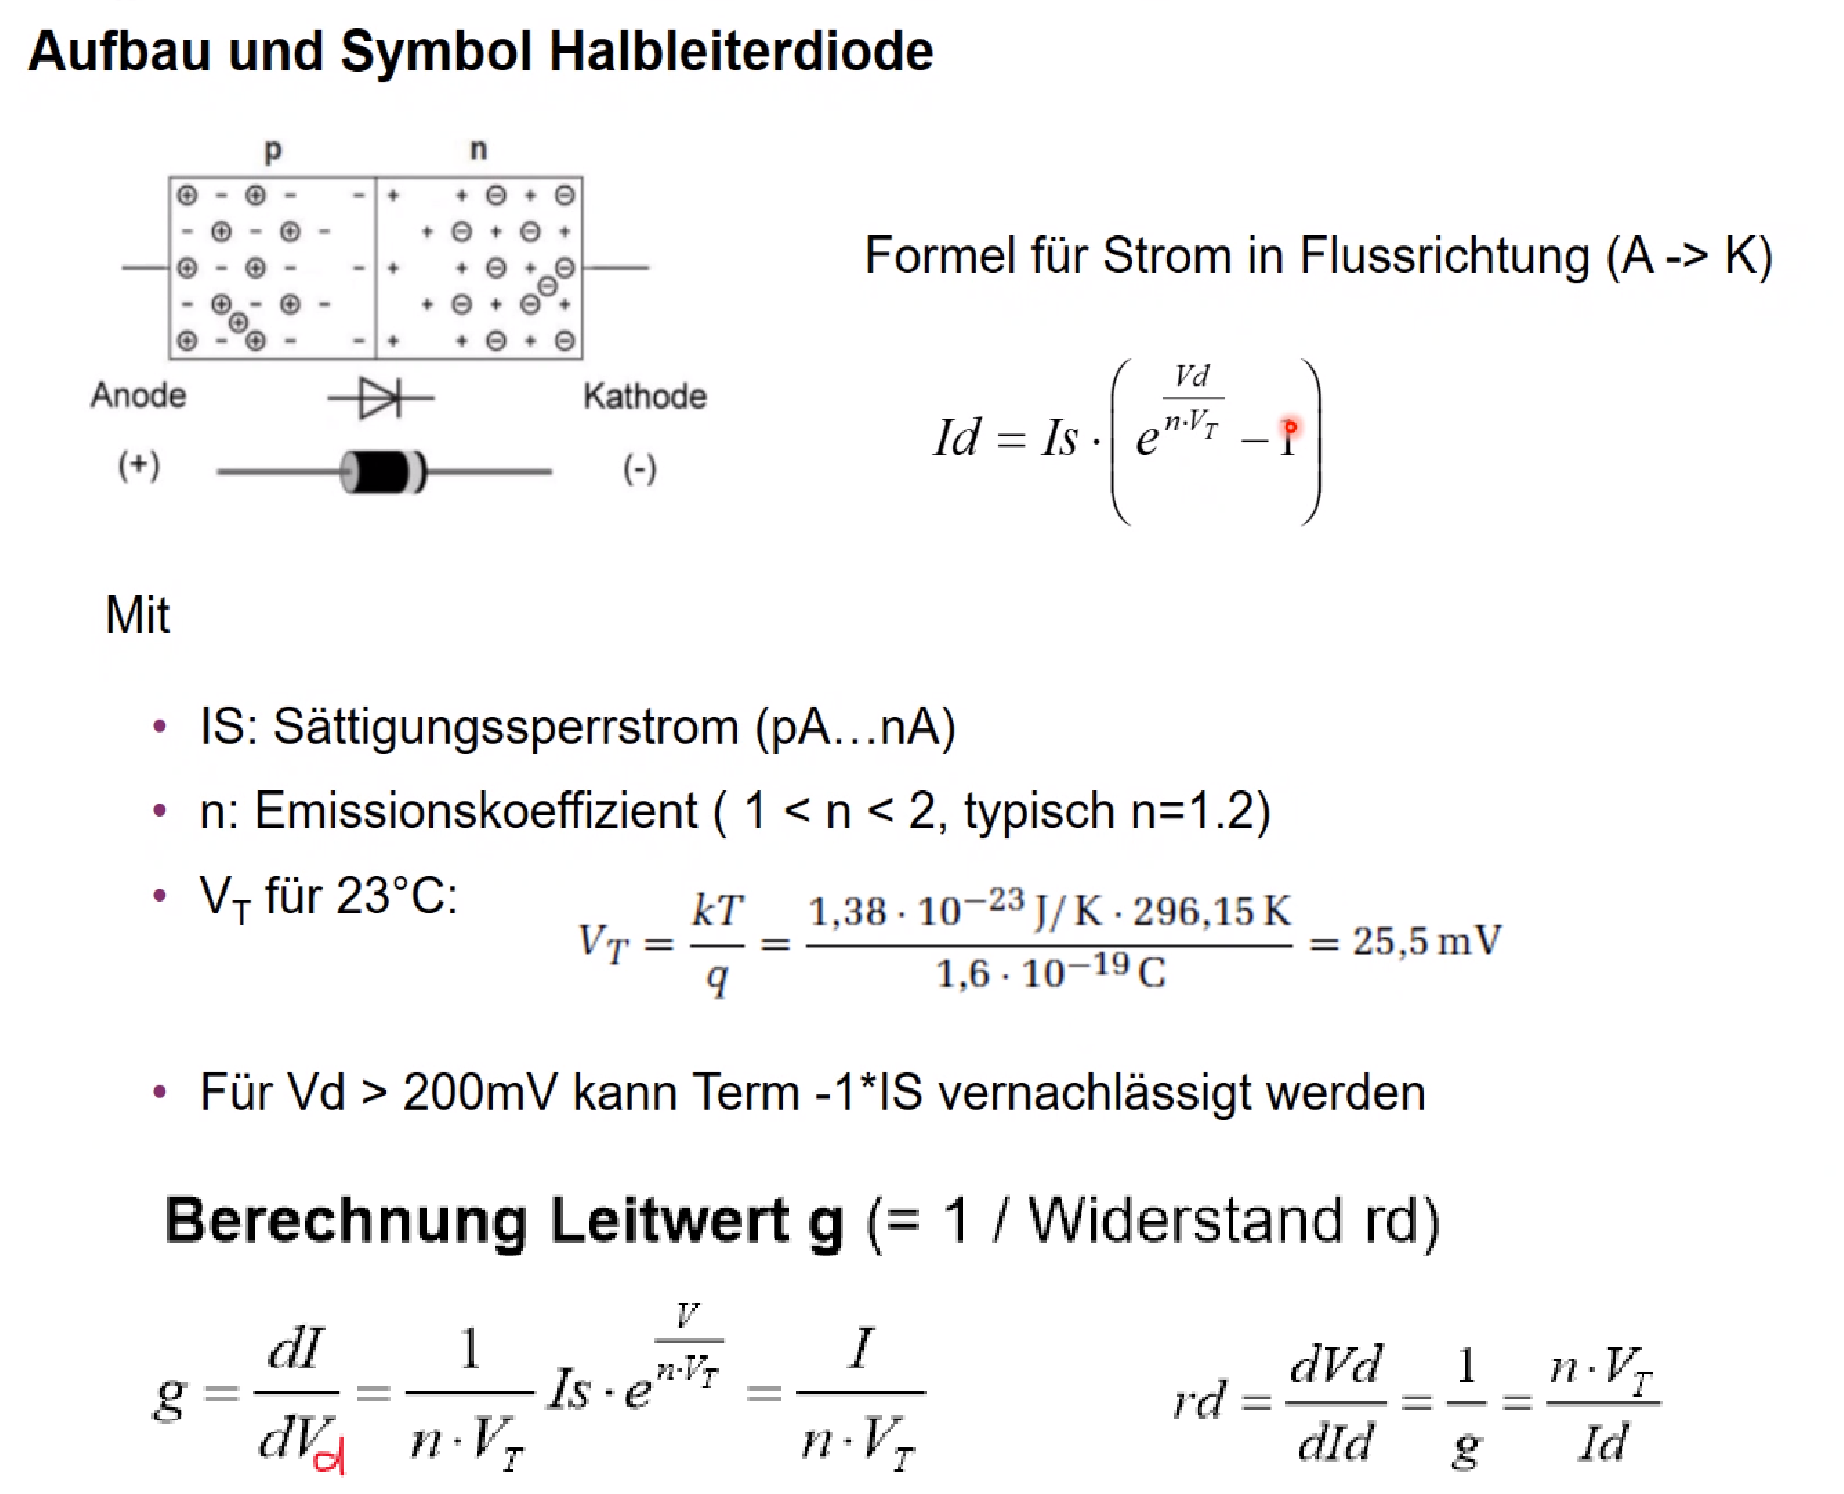
\includegraphics[width=\columnwidth]{Images/diode}

\subsection{Gleichrichter-Schaltung}
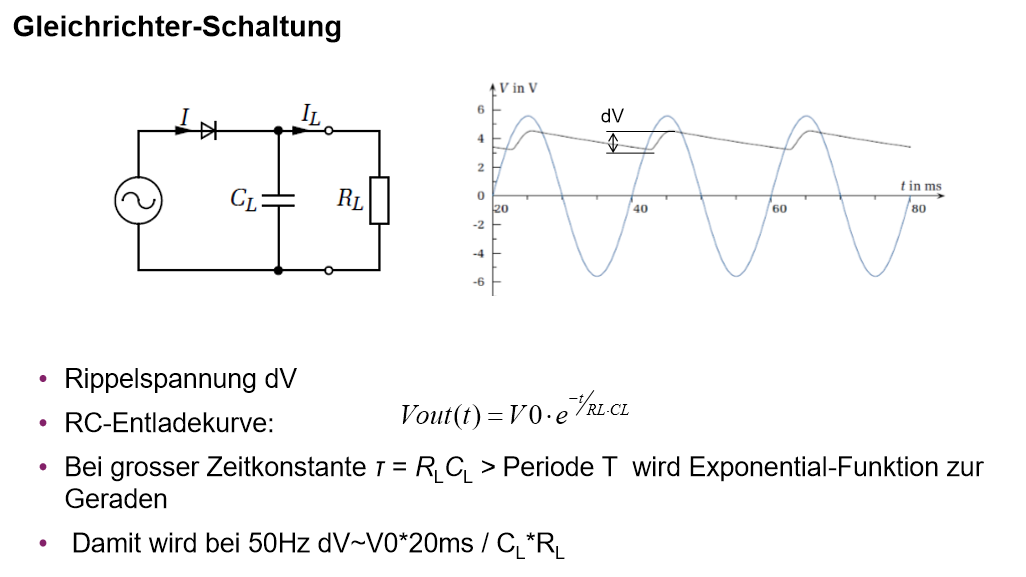
\includegraphics[width=\columnwidth]{Images/gleichrichter}


\subsection{Transistoren}
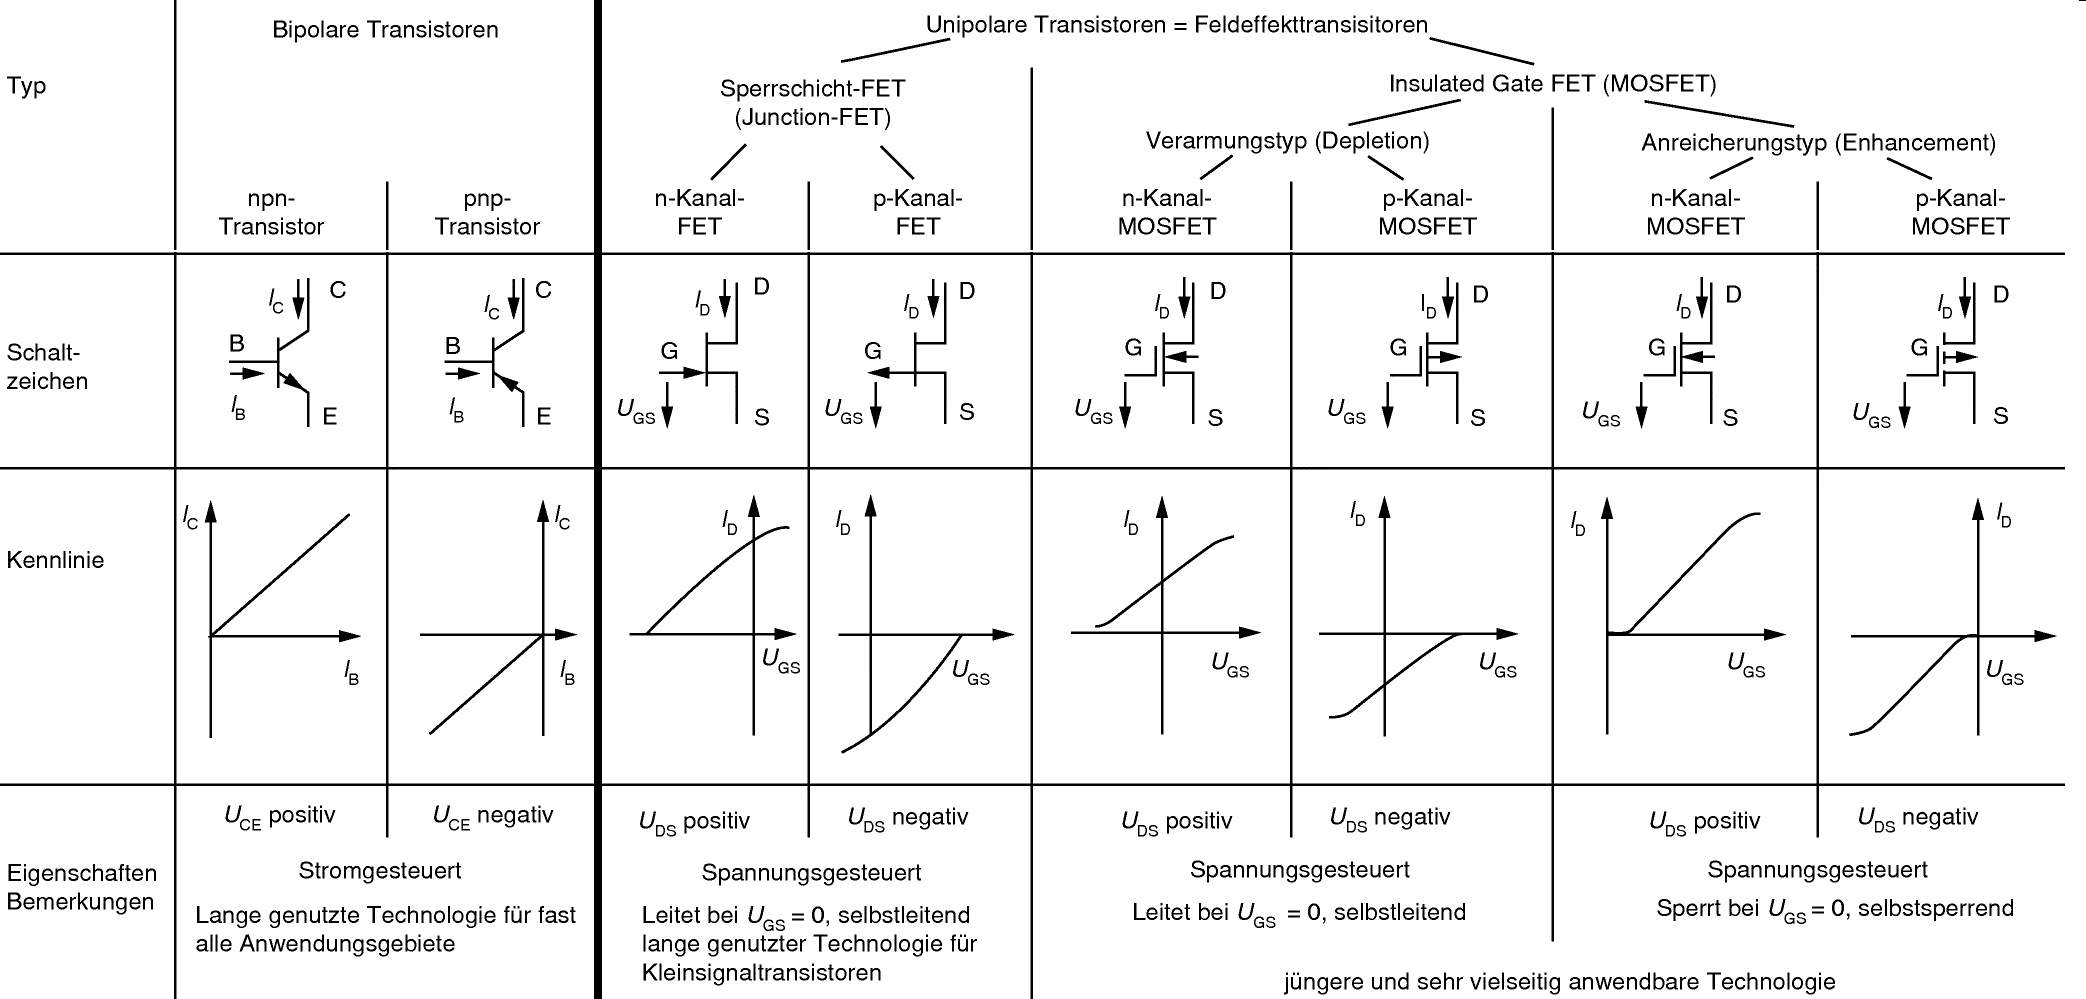
\includegraphics[width=\columnwidth]{Images/transistortypen}

\todo{Woche 10 nachschauen, Transistoren Teil 1..10}

\subsubsection{Bipolar-Transistor (BJT)}
\begin{center}
	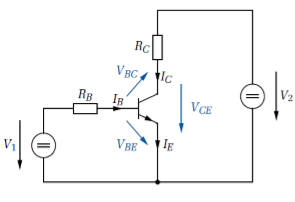
\includegraphics[width=0.5\columnwidth]{Images/bipolar}\\
	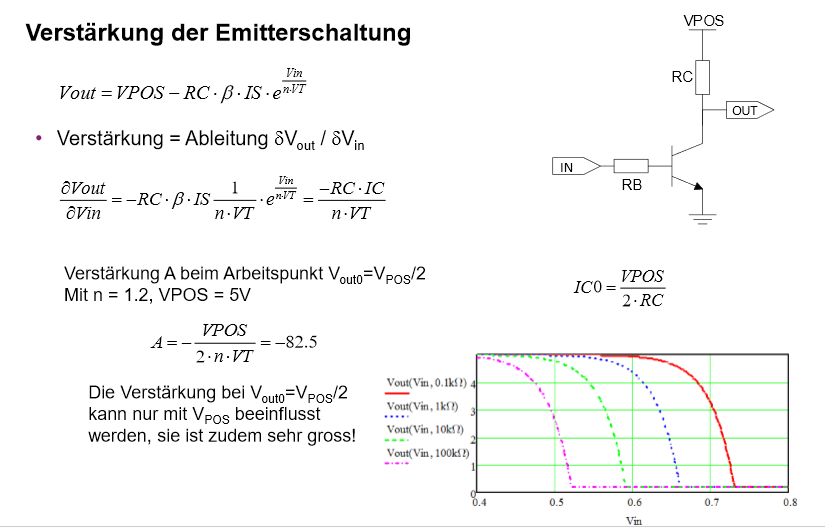
\includegraphics[width=\columnwidth]{Images/bipolar-formel3}\\
	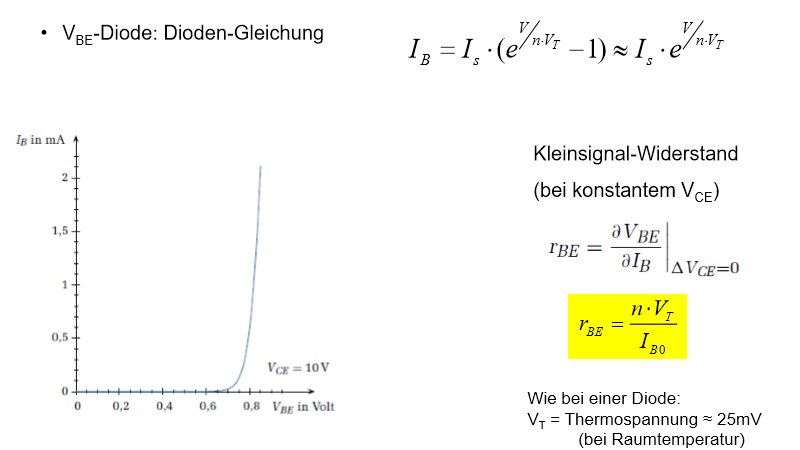
\includegraphics[width=\columnwidth]{Images/bipolar-formel}
\end{center}

\textbf{A/B und AB Verstärker}\\
% TODO: \usepackage{graphicx} required
\includegraphics[width=0.5\columnwidth]{Images/verstärker-typen}\\
% TODO: \usepackage{graphicx} required
\includegraphics[width=\columnwidth]{Images/verstärker-typen1}\\
% TODO: \usepackage{graphicx} required
\includegraphics[width=\columnwidth]{Images/verstärker-typen2}

\subsubsection{Feld-Effekt-Transsistoren (FET)}
% TODO: \usepackage{graphicx} required
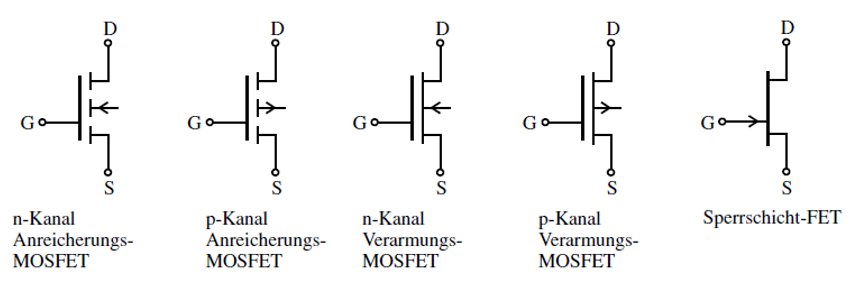
\includegraphics[width=\columnwidth]{Images/fet-typen}
